\documentclass[11pt]{article}
\usepackage[margin=1in]{geometry}
\usepackage{fontspec}
\usepackage{hyperref}
\usepackage[numbers,square]{natbib}
\usepackage{amsmath}
\usepackage{graphicx}
\usepackage{longtable}
\setmainfont{TeX Gyre Termes}
\begin{document}
\title{Fixed citation source - software acceptance}
\maketitle
\section{Other software source}
G09 software acceptance slot 1: this author note fills a template slot only; no scientific claim or external source is asserted.

\par\noindent\begin{minipage}{\linewidth}
\par\noindent\textbf{software-only-table.csv}\par\smallskip\noindent
\begingroup\small
\setlength{\tabcolsep}{3pt}
\begin{tabular}{|p{\dimexpr.98\linewidth/3-2\tabcolsep-4\arrayrulewidth/3\relax}|p{\dimexpr.98\linewidth/3-2\tabcolsep-4\arrayrulewidth/3\relax}|p{\dimexpr.98\linewidth/3-2\tabcolsep-4\arrayrulewidth/3\relax}|}
\hline
SOFTWARE\_FIXTURE & fictional\_value & qualification \\ \hline
alpha\_demo & 1 & Software rendering test only; no scientific measurement \\ \hline
beta\_demo & 2 & Software rendering test only; no scientific measurement \\ \hline
\end{tabular}
\endgroup
\end{minipage}\par
\par\noindent\begin{minipage}{\linewidth}\centering
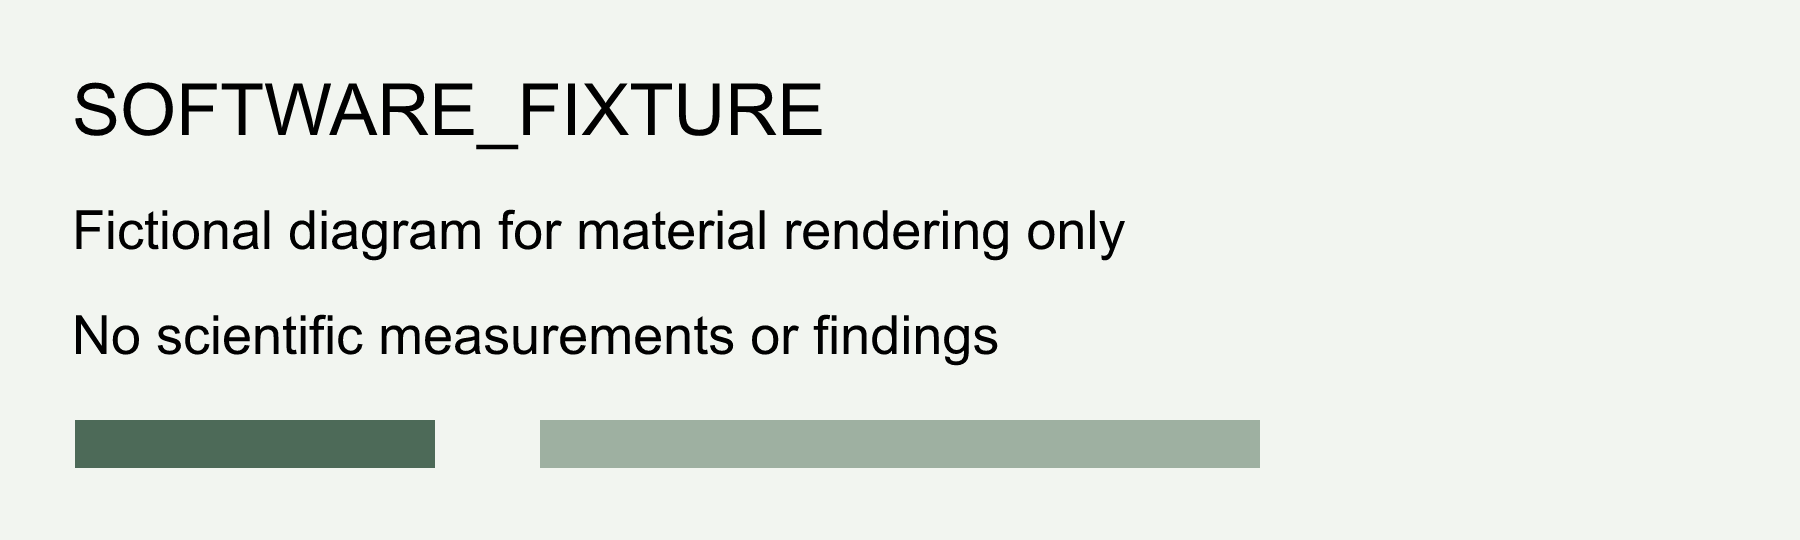
\includegraphics[width=\linewidth,height=.65\textheight,keepaspectratio]{material-asset_65e4b91ba806497e9afd0c7c514c7d1b-render.png}
\par\small software-only-figure.svg
\end{minipage}\par
\subsection{Introduction}
Beta software original paragraph. Keep this second paragraph's original source and conditions; no scientific claim is asserted. \citep{evidence_b5348fa59b3948ae9540b75a33ca9bd9} \citep{evidence_3a2639ee8b5e432aafd7e3743c825f33}

SOFTWARE\_FIXTURE: Check original sources only and preserve their original conditions without asserting any scientific claim; retain both original source-only and source-condition boundaries in this shared sentence and in their separate sentences. \citep{evidence_b5348fa59b3948ae9540b75a33ca9bd9} \citep{evidence_6b169de2b78d452f919391b00916f2c8} Check original sources only; no scientific claim is asserted. SOFTWARE\_FIXTURE C-MANY author clarification: preserve this source-only restriction in the shared sentence and in the separate source-check sentence. \citep{evidence_b5348fa59b3948ae9540b75a33ca9bd9} \citep{evidence_6b169de2b78d452f919391b00916f2c8} G09 software boundary: preserve the original sources and their conditions; no scientific claim is asserted. SOFTWARE\_FIXTURE C-MANY author clarification: retain this original boundary in the shared sentence and in the separate source-condition sentence.

G09 software acceptance slot 2: this author note fills a template slot only; no scientific claim or external source is asserted.

\subsection{Software source section 3}
G09 software acceptance slot 3: this author note fills a template slot only; no scientific claim or external source is asserted.

\subsection{Software source section 1}
G09 software acceptance slot 9: this paragraph preserves the original empty section in the generated workflow; no scientific claim is asserted.

\subsection{Software source section 2}
G09 software acceptance slot 5: this author note fills a template slot only; no scientific claim or external source is asserted.

\subsection{Software source section 3}
G09 software acceptance slot 6: this author note fills a template slot only; no scientific claim or external source is asserted.

\subsection{New section}
G09 software acceptance slot 7: this author note fills a template slot only; no scientific claim or external source is asserted.

G09 software acceptance slot 8: the original empty paragraph is retained and filled for this workflow test; no scientific claim is asserted.

\bibliographystyle{unsrtnat}
\bibliography{references}
\end{document}
